\documentclass{article}
\usepackage{comment}
\usepackage{graphicx}
\usepackage{hyperref}
\hypersetup{
    colorlinks,
    citecolor=black,
    filecolor=black,
    linkcolor=black,
    urlcolor=black
}

\title{NEA - Group Creator for School Projects}
\author{Amelie Machin}
\date{}

\begin{document}

\maketitle
\tableofcontents

\section{Analysis}
\subsection{Problem statement}
To form the perfect grouping for a group project within a school, many factors need to be taken into 
consideration to prevent students from feeling incapable of completing the project. These factors include skills of the students, skills 
required by the project, and number of students in the group.   

This project aims to create a tool to aid teachers in ensuring the students are separated into groups 
where the students are best able to get along and combine their individual skills to achieve their 
project’s aims. The user can input data about student relations and skills, data about the projects' 
skill requirements and group sizes and the program will output an optimal set of groups in the form of a table on a GUI to present the results in a readable way and an option to export the data as a CSV.

This program will not find, assume, or generate information about the students or project, it will 
only work with the data inputted to assign a group of students to a project.

Students will also benefit from this tool as they would be able to apply their skills to a project 
in a group of people they can enjoy time with, rather than being stuck on a project they have no 
interest in with people they do not get along with.

\subsection{Research}

\subsubsection{Sources of inspiration}
\begin{enumerate}
    \item\href{https://www.classtools.net/random-group-generator/}{Random group generator from ClassTools.net}:
    \begin{figure}[hb]
        \centering
        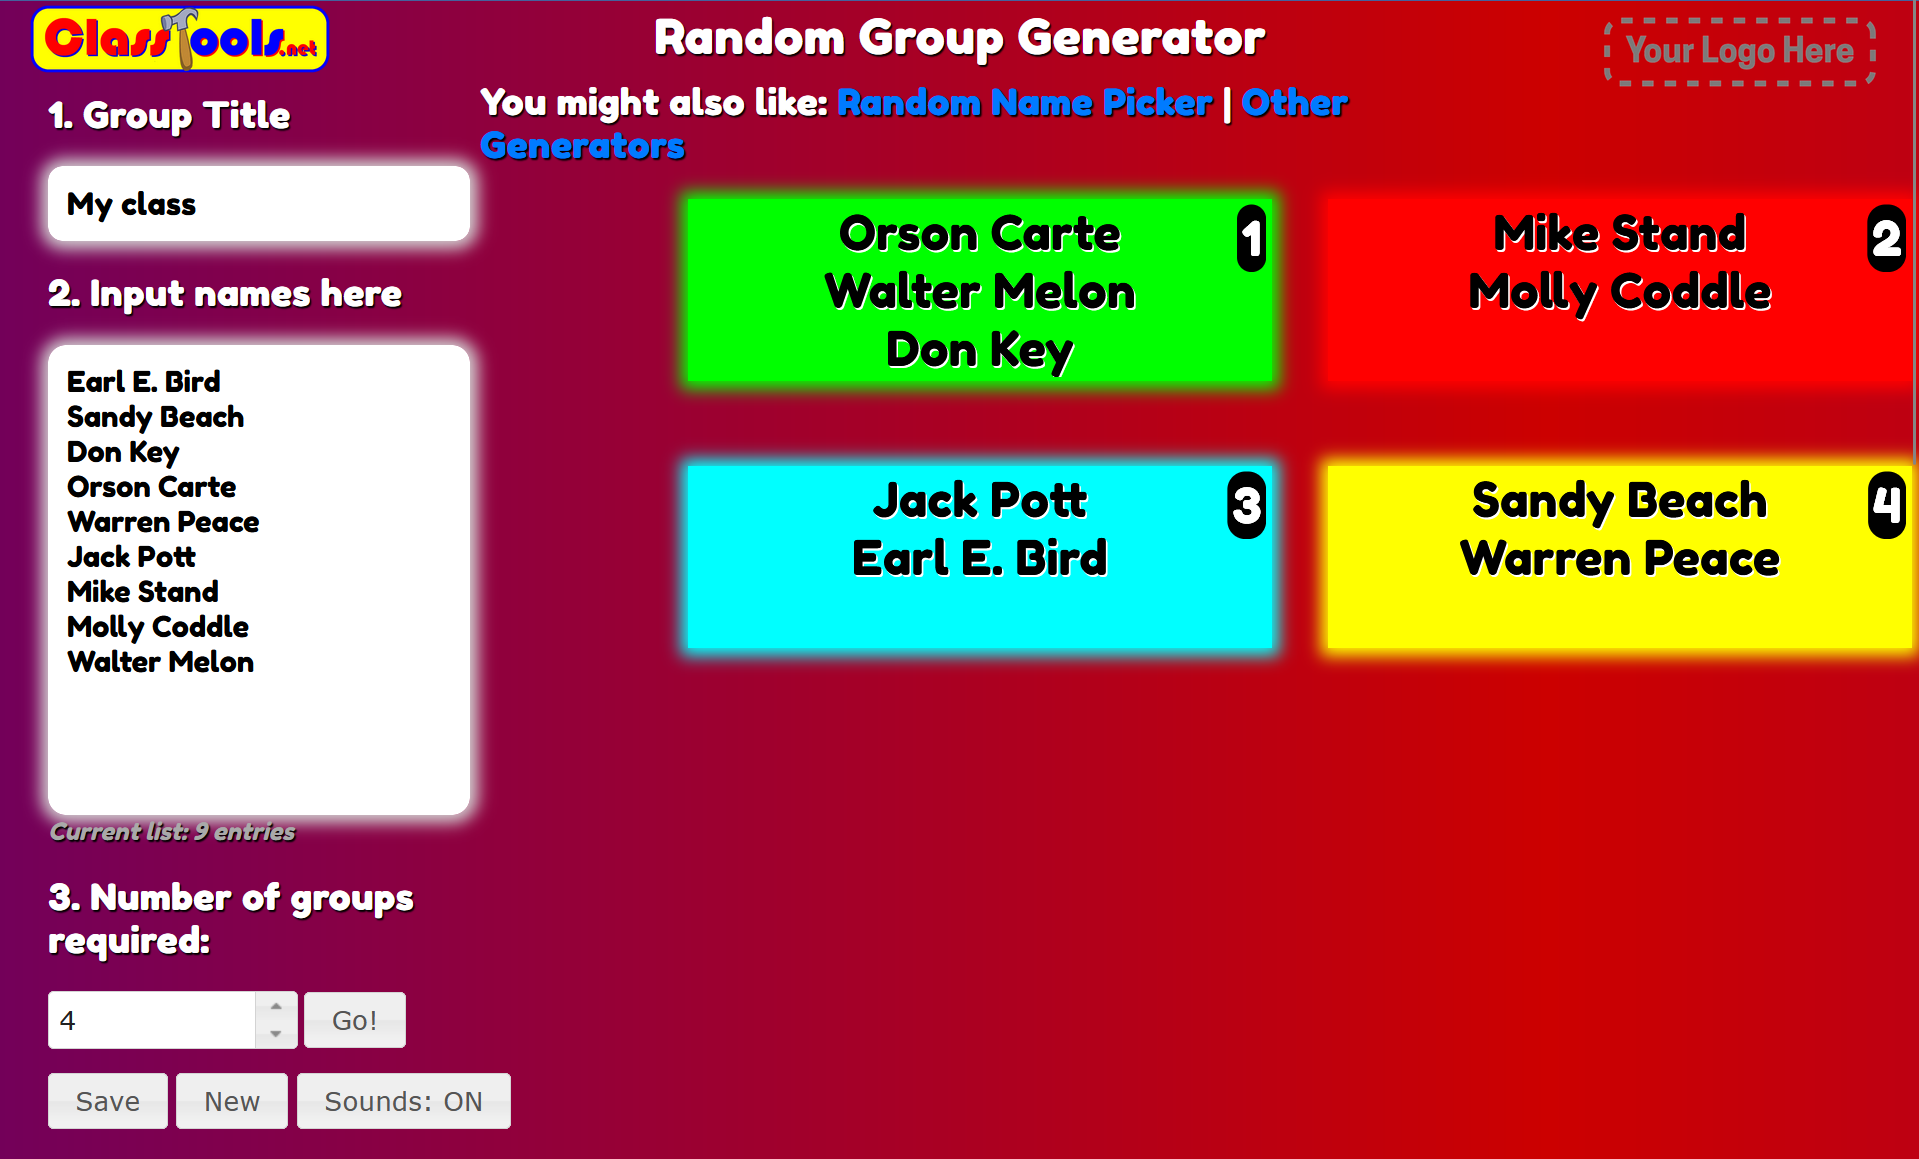
\includegraphics[width=0.5\linewidth]{Figures/classtools.png}
        \caption{ClassTools's random group generator tool with inputs and outputs visible on the same page}
    \end{figure}
    This tool is used frequently by my teachers to create random groups for group activities. The GUI 
    is very simple to use as there is little data that needs to be entered, so can all fit down the 
    left of the screen. The output is very easy to read as each group is visually separated using 
    both coloured boxes and numbering. However, this tool is too simple because it lacks any way to 
    group with conditions, which is part of my scope, as they are purely randomised. This means that 
    teams could quit often be unfairly balanced in terms of skill, or group students together that 
    are known to not work well together. The teacher's only option to solve this is to re-roll until 
    the output is suitable enough for the task manually. This gave me the idea for the algorithm to 
    be the simulation of this re-rolling and selection of optimal outputs.
    \item\href{https://www.keamk.com/random-team-generator}{keamk}:
    \begin{figure}[ht]
        \centering
        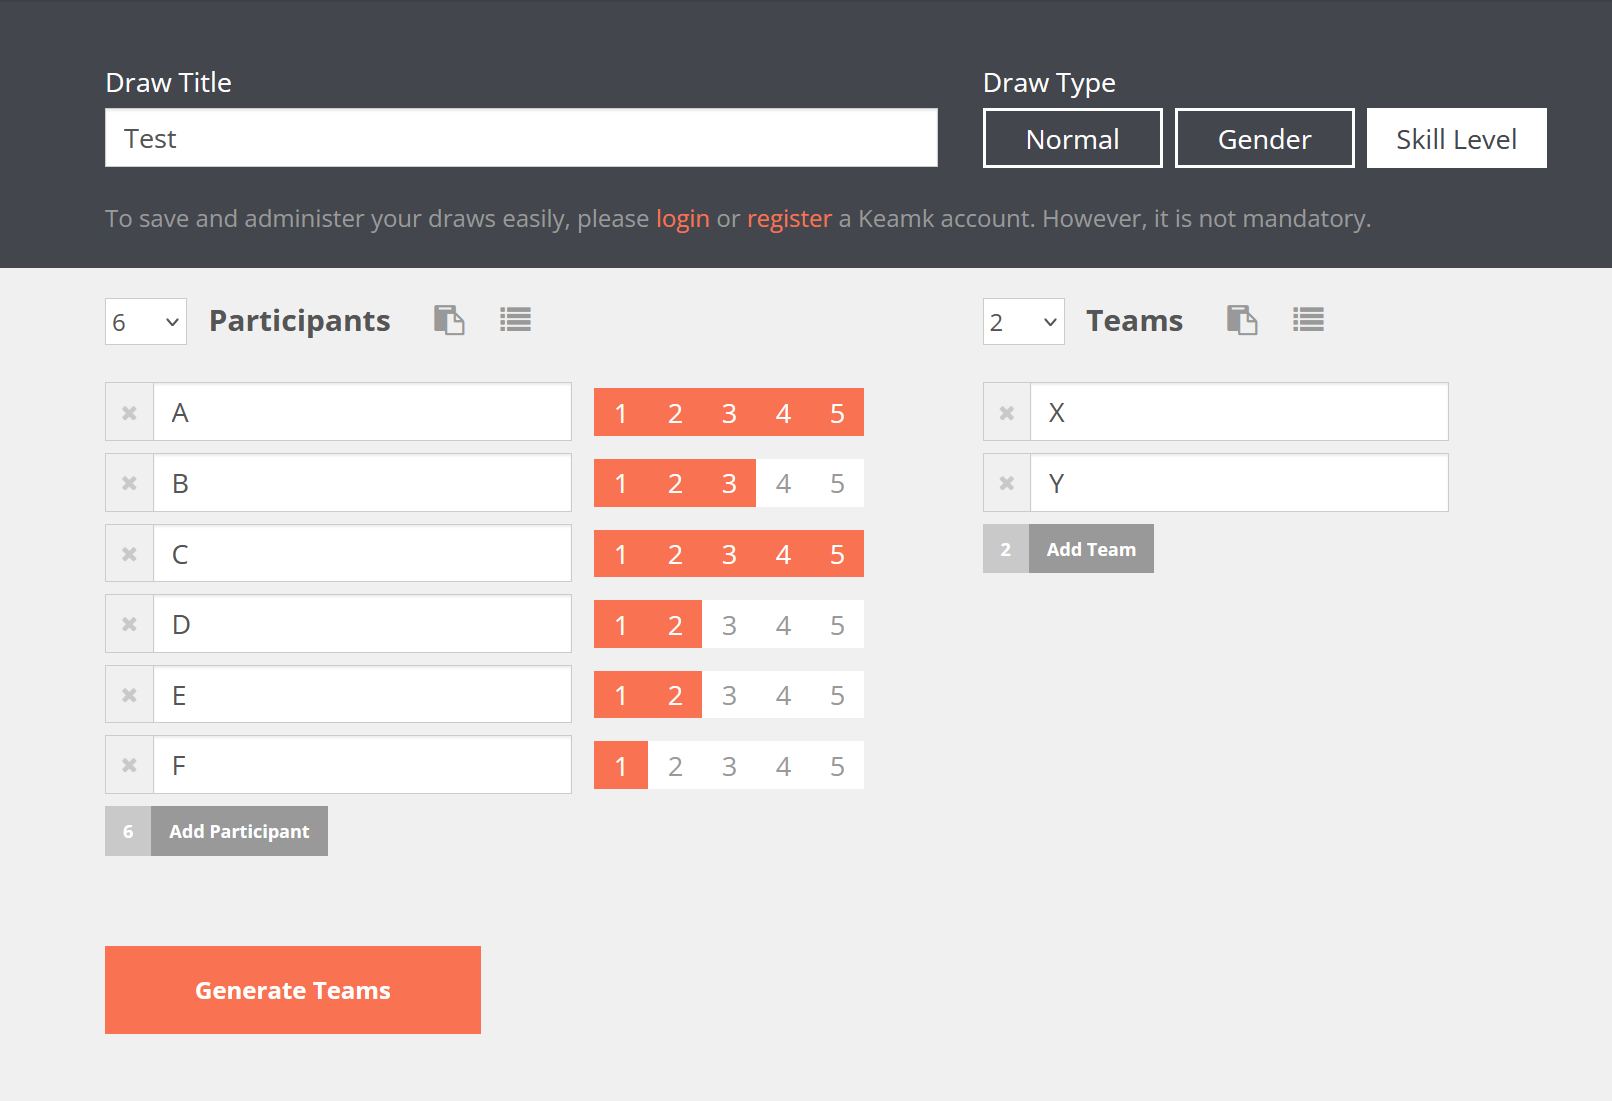
\includegraphics[width=0.5\linewidth]{Figures/keamkInput.png}
        \caption{Keamk's menu for inputting data}
    \end{figure}
    \begin{figure}[ht]
        \centering
        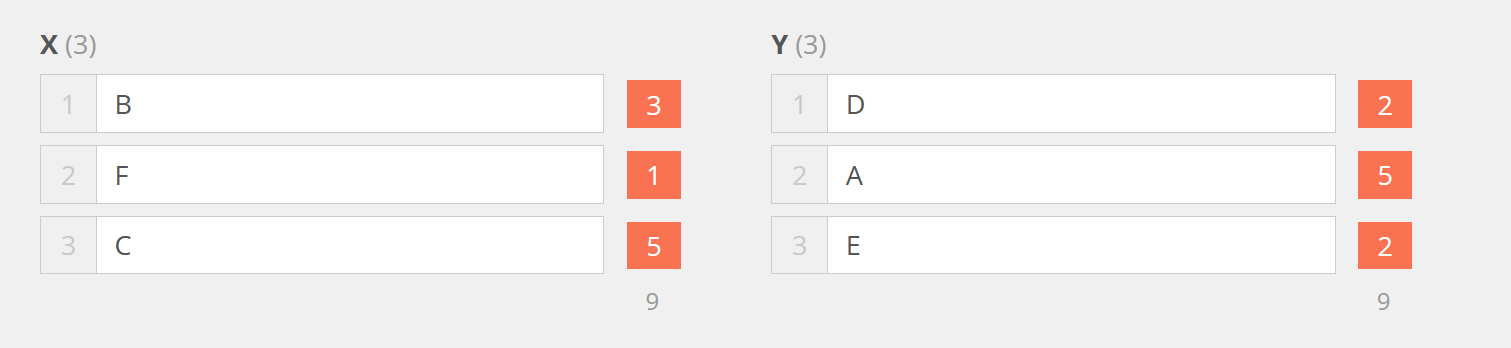
\includegraphics[width=0.5\linewidth]{Figures/keamkOutput.png}
        \caption{Keamk's outputs}
    \end{figure}
    This tool creates groups that all have a balanced level of skill. I like how the skill level is 
    inputted as a rating between 1-5 as this is intuitive for the user. I also like the extra details 
    that are outputted, such as how many are in each group next to the group name and the skill levels 
    next to each individual. Furthermore, the option to go back, make small changes to the data inputted and get new groupings 
    was very quick and useful.
    However, this tool can only create balanced groups, not groups with 
    different objectives as is in my scope, and there is no way to assign a certain number of 
    participants to each group, as the program puts the same number (or one away) of participants 
    in each group.
\end{enumerate}

\subsubsection{Algorithm}
I have researched into representing students and projects into bipartite graphs, and then using 
matching algorithms such as the alternate path algorithm to join students to projects. However, this 
will only match one student to one project, not groups so is not suitable. I then researched applying 
the algorithm repeatedly to graphs with randomised students, but this means that some students will 
never be joined into a group purely based on chance and that the groups formed are such that each 
individual is best for the project, not that the overall group is best suited for the project, so 
teamwork will not as high as it could be. I then researched using a grouping algorithm, such as 
\href{https://help.feedbackfruits.com/hc/en-us/articles/23527084211346-Group-Formation-Algorithm-Explainer}{explained here} 
to create similar groups then using bipartite matching algorithms to match them. However this only 
creates groups with similar skill sets, not skill sets that very based on the project.
\newline
I am currently looking into a genetic algorithm where each individual is made up of a possible 
solution and the fitness score is a calculation between how suited each group is to the assigned 
project. The solutions with lower fitness scores are discarded and the higher ones crossover to 
form new solutions. Some of these solutions then have random mutations, which involve swapping of 
students between projects. New fitness scores are calculated and the process repeats a predetermined 
number of times.

\subsubsection{Inputting data}
For the inputting of data, I have decided that it can be inputted through txt and csv files, through databases, manually  on the GUI, or any combination of those methods. This is because the data for different individuals and different projects could be stored in different ways within the same system, and manual tweaks may be needed by the user to ensure all data is as is needed by the application. I will also include the option to import the data from an Excel spreadsheet at the request of my third party.

\subsubsection{Accounts}
I have decided against implementing an account system because I don't think it will provide any value to the program. Accounts are
typically used for ensuring data can only be accessed by the users with the correct permissions. As this program will be designed to
be run locally, all the data will be stored and only accessible on the machine the program was run on, so the OS can handle user security.
\begin{comment}
Another reason for accounts is allow users to access their data that has been stored by a third party, especially within a cloud to allow
for data to be quickly transferred between devices. I will implement a manual solution to this by allowing users to export and import all
the data the program stores and the user can handle that data transfer manually. 
\end{comment}

\subsubsection{Internal data storage}
I chose to store the data about the students and projects in their own classes, that are aggregated within an 'individual' class. The student and project classes contain their names, skills and the project will have the recommended group size. The individual will contain a project object, student objects, and current fitness score as well as methods for calculating fitness scores, crossover with other individuals, and mutations.
This keeps the attributes and methods stored together in the program to make the code easier to read and understand by a programmer.

\subsubsection{External data storage}
I have researched into whether information about projects and students should be stored somewhere, and if so, how. I have concluded that they should be stored in relational databases that are accessible and modifiable by entering the details into the graphical interface, which are passed as parameters into SQL statements. These can then be loaded as a list of checkboxes that can be selected and deselected by the user for that run.

I chose to store the data because being able to make minor changes to the data and then re-running the program quickly is a very valuable feature that could save users' time and energy as they would not have to go through the entire process of entering every piece of data just for small changes to some of the data. This feature is present in keamk's grouping tool, and I found it very useful in my testing.

I chose databases to store the data because I have more experience working with relational databases and SQL then any other form of data storage, such as in files. The data is structured so databases would allow for efficient access and modification of specific entries.

\subsubsection{GUI library}
\begin{figure}[ht]
    \centering
    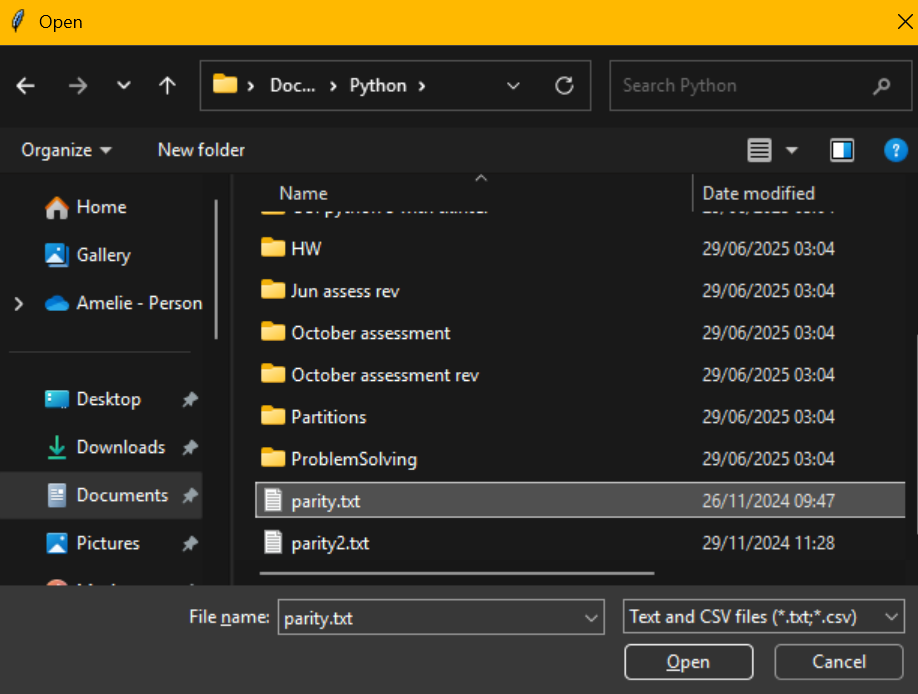
\includegraphics[width=0.5\linewidth]{Figures/fileDialog.png}
    \caption{Tkinter's file dialog, configured to only show .txt and .csv files}
    \label{fig:tkfiles}
\end{figure}
Between the two main python GUI libraries, pygame and Tkinter, I chose Tkinter because of the 
larger library of classes of pre-made, customisable widgets that can be used more easily to produce 
a simple, easy-to-use tool, such as a dialog that allows users to graphically navigate through their 
files to find their data file [Fig.\ref{fig:tkfiles}]. On the other hand, with my prior experience 
with pygame, I have found it to be more suited towards building games and graphically-complex tools, 
which is not what I am aiming for in this project. I am aiming to have a GUI that is quick and simple 
to create and edit, and has user-friendly features for inputting, editing, and reading data. I also 
have more experience with Tkinter, which will reduce the amount of time I spend on the GUI and allow 
me to focus on developing and improving the grouping algorithm. 


\subsection{Dialogue}
My third party is Dr Ed Horncastle, the lead teacher for the Exeter Mathematics Certificate (EMC) at 
my school, which is where groups of 3 or 4 students work together on research projects set by 
University academics or companies. He is suitable because he has to make these groups based on the 
skills of the students and match them to projects every year, so he has a thorough understanding of 
how this tool could work and would benefit from using this tool. I interviewed him and asked him the following questions:
\begin{enumerate}
    \item What is the current process for creating EMC groups? 
        \begin{itemize} \item All the metrics to consider are gathered into a spreadsheet and then groups are formed by hand. \end{itemize}
    \item What are these metrics?
        \begin{itemize} \item Students' own choice \item There must be a mix of genders \item The projects must be relevant to the A-level studies of that student. Someone who does not take computer science shouldn't be given a computer science based project\item Those that work hard and those that laze off more easily should be mixed together. If this is their first project, this is inferred from GCSE results, otherwise it is based off the results of previous projects. \item Special educational needs \item Timetabling restrictions \item Students do not get put into groups with others they have worked on projects with before \end{itemize}
    \item How are the student choices measured?
        \begin{itemize} \item For some of the projects, the students give their top 3 choices of projects. Starting with the least popular project, the groups are formed by trying to minimise the sum of the positions the student's ranked the project in. \end{itemize}
    \item How is the data about the students and projects currently stored?
        \begin{itemize} \item Excel spreadsheet \end{itemize}
    \item How would you prefer to input the data?
        \begin{itemize} \item Student choices from a Microsoft Form and all other data from a Excel spreadsheet \end{itemize}
    \item How much data and in what format do you think the data should be outputted?
        \begin{itemize} \item In tables with the project name, student names and summaries of information about each group such as gender ratio, how many take computer science or physics, and how many have special education needs. \item As a simplified register in alphabetical order \end{itemize}
    \item How useful would storing project/student details locally, that can be loaded when needed, be for you?
            \begin{itemize} \item Very \end{itemize}
    \item Are there any other features that would be useful for this tool to include?
        \begin{itemize} \item Some extra features that could be added is timetabling for what order the projects are presented in, and itinerary for group trips out of school. \end{itemize}
\end{enumerate}

\subsection{Objectives}
\begin{enumerate}
    \item (Entering the data)
    \item (processing the data)
    \item (outputting the data)
\end{enumerate}

\subsection{Modelling}
\begin{figure}[hb]
    \centering
    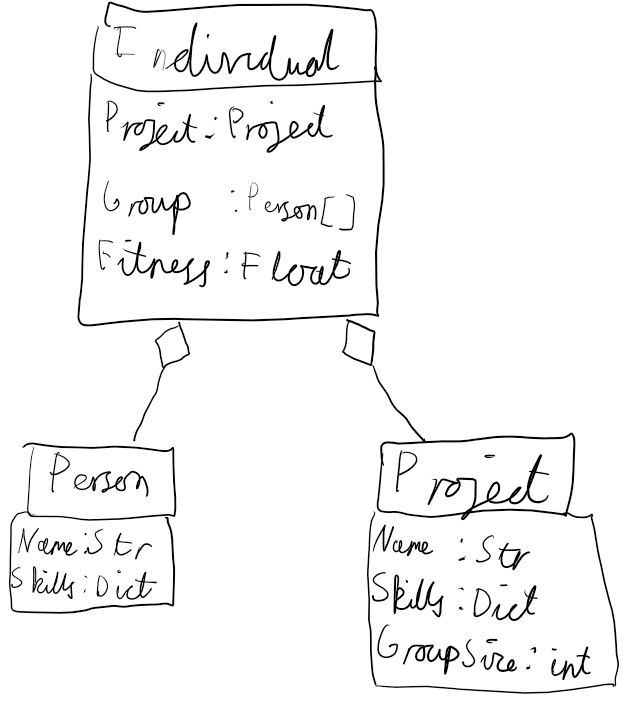
\includegraphics[width=0.7\linewidth]{Figures/classAnalysis.png}
    \caption{Class diagram showing relationship between the classes within the program and their attributes}
\end{figure}
\end{document}
